
\section{Mass and tracer transport}
\label{sc:glissade-transport}

We wish to solve the continuity or transport equation for the ice thickness:

(Insert correct equation)

\begin{equation}
  \label{gliss.eq.transport_mass}
  \frac{\partial H}{\partial t} + \nabla \cdot (H {\bf U}) = \dot{b},
\end{equation}

\noindent
where ${\bf U}$ is the vertical average velocity and $\dot{b}$ is the 
mass balance at the upper and lower surfaces.
Equation (\ref{gliss.eq.transport_mass}) describes the conservation of
ice mass under horizontal transport.  
Mass conservation is equivalent to volume conservation with the assumption
of uniform density.

There is a similar conservation equation for internal energy:

\begin{equation}
  \label{gliss.eq.transport_energy}
  \frac{\partial{H T}}{\partial t} + \nabla \cdot (H T {\bf U}) = 0,
\end{equation}

where $T$ is the internal ice temperature, and we have neglected other terms in the
energy equations (e.g., vertical diffusion and internal dissipation, which Glissade handles
separately).
Advection of tracers other than temperature (e.g., internal water fraction and ice age)
can be described with similar equations.


Once the IR algorithm has been applied to each ice layer, the new layer thicknesses
generally do not have the desired spacing in $\sigma$ coordinates.
A vertical remapping step is needed to move ice thickness (and associated
tracers) between layers to conserve volume and energy.

Glissade has two transport schemes: a basic first-order
upwind scheme and a more complex incremental remapping (IR) scheme.
The IR scheme \citep{Dukowicz2000, Lipscomb2004} 
was originally implemented in the Los Alamos sea ice model, CICE,
and has been simplified and adapted for CISM.  

\subsection{Incremental remapping}
\label{sc:incremental_remapping}

The remapping scheme has several desirable features:
\begin{itemize}
\item It conserves the quantity being transported (volume or energy).
\item It is non-oscillatory; that is, it does not create spurious
      ripples in the transported fields.
\item It preserves tracer monotonicity.  That is, it does not create
      new extrema in the temperature field; the values
      at time~$m+1$ are bounded by the values at time~$m$.
\item It is second-order accurate in space and therefore is
      less diffusive than first-order schemes (e.g., upwind).
      The accuracy may be reduced locally to first order to preserve monotonicity.
\item It is efficient for large numbers of tracers.
      Much of the work is geometrical and is performed
      only once per grid cell instead of being repeated for each
      quantity being transported.  (This is more of an issue for CICE than
      for CISM, but for some application it might be desirable to transfer 
      additional tracers in CISM.)
\end{itemize}
The time step is limited by the requirement that trajectories
projected backward from grid cell corners are confined to the four
surrounding cells; this is what is meant by incremental
remapping as opposed to general remapping. This requirement leads to a 
CFL-like condition, 

\begin{equation}
  \frac{\max|{\bf u}|\Delta t} {\Delta x} \leq 1 
\end{equation}

For highly divergent velocity fields the maximum time
step must be reduced by a factor of two to ensure that
trajectories do not cross.  However, ice-sheet velocity fields
usually have small divergences per time step relative to the grid size.

The remapping algorithm can be summarized as follows:
\begin{enumerate}
\item Given mean values of the ice thickness and tracer fields in each
      grid cell, construct linear approximations of these fields.
      Limit the field gradients to preserve monotonicity.
\item Given ice velocities at grid cell corners, identify departure
      regions for the fluxes across each cell edge.  Divide these
      departure regions into triangles and compute the coordinates
      of the triangle vertices.
\item Integrate the area and tracer fields over the departure triangles to obtain
      the area, volume, and energy transported across each cell edge.
\item Given these transports, update the state variables.
\end{enumerate}
These steps are carried out for each of $nz-1$ ice layers, as described below.

%%%%%%%%%%%%%%%%%%%%%%%%%%%%%%%%%%%%%%%%%%%%%%
\subsubsection{Reconstructing area and tracer fields}
\label{sc:glissade-IR-reconstruct}

First, using the known values of the state variables, the ice thickness
and tracer fields are reconstructed in each grid cell as linear
functions of $x$ and $y$. For each field we compute the value at
the cell center, along with gradients in the
$x$ and $y$ directions. The gradients are limited to preserve
monotonicity.  When integrated over a grid cell, the reconstructed
fields must have mean values equal to the known state variables,
denoted by $\bar{H}$ for ice thickness and $\tilde{T}$ for temperature.

Consider first the ice thickness in a given layer. We contruct a field
field $H({\bf{r}})$ whose mean is $\bar{H}$, where $\mathbf{r} = (x,y)$ 
is the position vector relative to the cell center. That
is, we require

\begin{equation}
  \label{gliss.eq.IR_mean_thickness}
  \int_A H \, dH = {\bar H} \, A,
\end{equation}

\noindent
where $A=\int_A dA$ is the grid cell area.
Eq.~\eqref{gliss.eq.IR_mean_thickness} is satisfied if $H({\bf r})$ has the form

\begin{equation}
  \label{gliss.eq.IR_recon_thickness}
  H({\bf r}) = \bar{H} + \alpha_H \left<\nabla H\right> \cdot ({\bf r}-{\bf \bar{r}}),
\end{equation}

\noindent
where $\left<\nabla H\right>$ is a centered estimate of the thickness
gradient within the cell, $\alpha_H$ is a limiting coefficient that
enforces monotonicity, and ${\bf \bar{r}}$ is the cell centroid:
\[{\bf \bar{r}} = \frac{1}{A} \int_A {\bf r} \, dA.\]
On CISM's structured rectangular grid we have $\mathbf{\bar{r}} = 0$;
thus $H(\mathbf{bar{r}}) = \bar H$.


%${\bf \bar{r}}$, $\overline{x} = \int_A x \, dA / A$ and
%$\overline{y} = \int_A y \, dA / A$, are evaluated using the triangle
%integration formulas described in Section~\ref{subsubsec:integ_flux}.
%These means, along with higher-order means such as $\overline{x^2}$,
%$\overline{xy}$, and $\overline{y^2}$, are computed once and stored.

Next consider the ice temperature field in a layer of thickness $H$. 
The reconstructed temperature must satisfy

\begin{equation}
  \label{gliss.eq.IR_mean_temperature}
  \int_A H \, T \, dA = \bar{H} \, \tilde{T} \, A,    \\
\end{equation}

\noindent
where $\tilde{T} = T(\tilde{\bf r})$ is the temperature at the center of ice mass.
Eq. \eqref{gliss.eq.IR_mean_temperature} is satisfied when $T({\bf r})$ is given by

\begin{equation}
  \label{gliss.eq.IR_recon_temperature}
  T({\bf r}) = \tilde{T} + \alpha_T \left<\nabla T\right> \cdot
                                     ({\bf r}-{\bf \tilde{r}}),
\end{equation}

\noindent
where $\alpha_T$ is a limiting coefficient, and the center of ice mass
${\bf\tilde{r}}$ is given by

\begin{equation}
{\bf \tilde{r}} = \frac{1}{\bar H \, A} \int_A H \, {\bf r} \, dA.
\end{equation}

\noindent
Evaluating the integrals, we find that the components of ${\bf \tilde{r}}$ are
\begin{equation}
  \begin{split}
    \tilde{x} & = \frac{H_c \overline{x} + H_x \overline{x^2} + H_y \overline{xy}} {\bar{H}}, \\
    \tilde{y} & = \frac{H_c \overline{y} + H_x \overline{xy} + H_y \overline{y^2}} {\bar{H}}.
  \end{split}
\end{equation}

\noindent
From \eqref{gliss.eq.IR_recon_temperature}), the temperature at the cell center is given by
\[ T_c = \tilde{T} - T_x \tilde{x} - T_y \tilde{y}, \]
where ($T_x, T_y$ is the limited gradient of temperature.

We preserve monotonicity by van Leer limiting. If
$\bar{\phi}(i,j)$ denotes the mean value of some field in grid cell
$(i,j)$, we first compute centered gradients of $\bar{\phi}$ in
the $x$ and $y$ directions, then check whether these gradients
give values of $\phi$ within cell $(i,j)$ that lie outside the
range of $\bar{\phi}$ in the cell and its eight neighbors.  Let
$\bar{\phi}_{\max}$ and $\bar{\phi}_{\min}$ be the maximum and
minimum values of $\bar{\phi}$ over the cell and its neighbors,
and let $\phi_{\max}$ and $\phi_{\min}$ be the maximum and minimum
values of the reconstructed $\phi$ within the cell.  Since the
reconstruction is linear, $\phi_{\max}$ and $\phi_{\min}$ are
located at cell corners.  If $\phi_{\max} > \bar{\phi}_{\max}$ or
$ \phi_{\min} < \bar{\phi}_{\min}$, we multiply the unlimited
gradient by $\alpha = \min(\alpha_{\max}, \alpha_{\min})$, where

\begin{equation}
  \label{gliss.eq.IR_limited_gradient}
  \begin{split}
    \alpha_{\max} = (\bar{\phi}_{\max} - \bar{\phi}) / (\phi_{\max} -\bar{\phi}), \\
    \alpha_{\min} = (\bar{\phi}_{\min} - \bar{\phi}) / (\phi_{\min} -\bar{\phi}).
  \end{split}
\end{equation}

\noindent
Otherwise the gradient need not be limited.

%%%%%%%%%%%%%%%%%%%%%%%%%%%%%%%%%%%%%%%%%%%%%%
\subsubsection{Locating departure triangles}
\label{sc:glissade-IR-departure} 
The method for locating departure triangles is discussed in detail by 
\citet{Dukowicz2000}. The basic idea is illustrated in Figure ~\ref{fig:gliss.deparr}, 
which shows a shaded quadrilateral departure region whose contents are transported to
the target or home grid cell, labeled $H$. The neighboring grid
cells are labeled by compass directions: $NW$, $N$, $NE$, $W$, and
$E$.  The four vectors point along the velocity field at the cell
corners, and the departure region is formed by joining the
starting points of these vectors.  Instead of integrating over the
entire departure region, it is convenient to compute fluxes across
cell edges.  We identify departure regions for the north and east
edges of each cell, which are also the south and west edges of
neighboring cells. Consider the north edge of the home cell,
across which there are fluxes from the neighboring $NW$ and $N$
cells. The contributing region from the $NW$ cell is a triangle
with vertices $abc$, and that from the $N$ cell is a quadrilateral
that can be divided into two triangles with vertices $acd$ and
$ade$. Focusing on triangle $abc$, we first determine the
coordinates of vertices $b$ and $c$ relative to the cell corner
(vertex $a$), using Euclidean geometry to find vertex $c$. Then we
translate the three vertices to a coordinate system centered in
the $NW$ cell.  This translation is needed in order to integrate
fields (Section~\ref{sc:glissade-IR-integrate}) in the coordinate
system where they have been reconstructed
(Section~\ref{sc:glissade-IR-reconstruct}). Repeating this process for
the north and east edges of each grid cell, we compute the
vertices of all the departure triangles associated with each cell
edge.

\begin{figure}
  \label{fig:gliss.deparr}
  \centering
    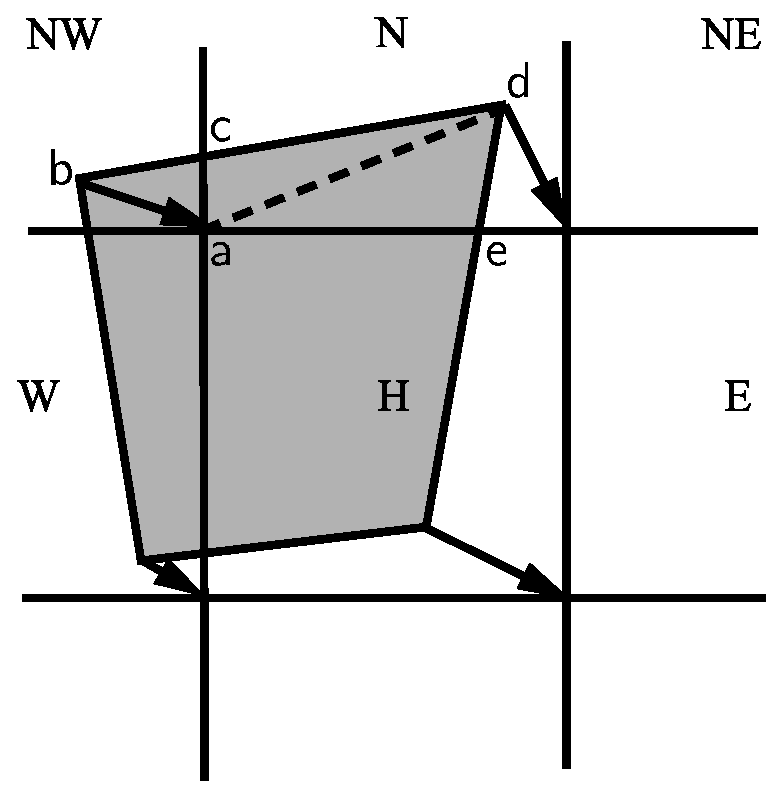
\includegraphics[width=0.5\columnwidth]{\dir/figs/deparr.eps}
    \caption{In incremental remapping, conserved
      quantities are remapped from the shaded departure region, a
      quadrilateral formed by connecting the backward trajectories
      from the four cell corners, to the grid cell labeled $H$.
      The region fluxed across the north edge of cell $H$ consists
      of a triangle ($abc$) in the $NW$ cell and a quadrilateral 
      (two triangles, $acd$ and $ade$) in the $N$ cell.}
\end{figure}

Figure~\ref{fig:gliss.triangles}, reproduced from \citet{Dukowicz2000}, shows all possible
triangles that can contribute fluxes across the north edge of a
grid cell.  There are 20 triangles, which can be organized into
five groups of four mutually exclusive triangles as shown in
Table~\ref{table:triangles}. In this table, $(x_1, y_1)$ and $(x_2,y_2)$ are the
Cartesian coordinates of the departure points relative to the
northwest and northeast cell corners, respectively.  The departure
points are joined by a straight line that intersects the west edge
at $(0,y_a)$ relative to the northwest corner and intersects the
east edge at $(0,y_b)$ relative to the northeast corner. The east cell
triangles and selecting conditions are identical except for a
rotation through 90 degrees.

\begin{figure}
  \label{fig:gliss.triangles}
  \centering
    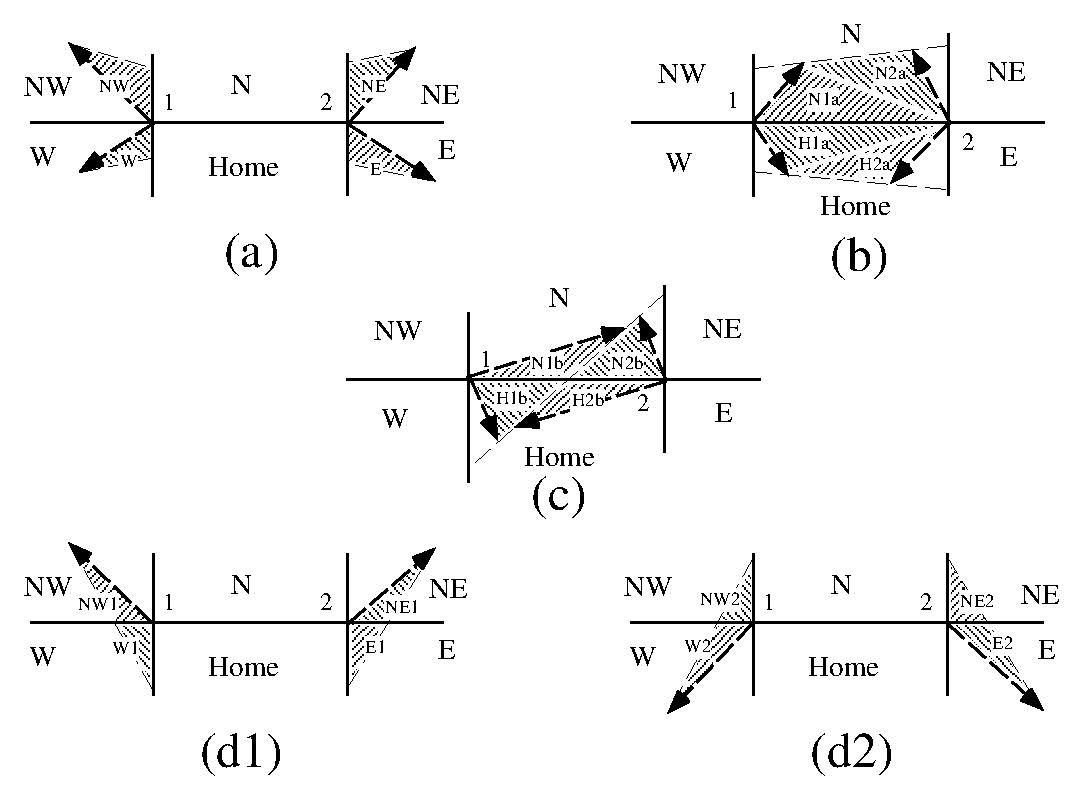
\includegraphics[width=0.7\columnwidth]{\dir/figs/triangles.eps}
  \caption{The 20 possible triangles that can
    contribute fluxes across the north edge of a grid cell.}
\end{figure}


%\newpage
\begin{table}
\begin{center}
\begin{tabular}{cccc}
\hline
Triangle  &  Triangle  &   Selecting logical                   \\
group     &   label    &   condition                           \\
\hline
          &        &            &                                       \\
1         &    NW      &  $y_a>0$ and $y_1\geq0$ and $x_1<0$ \\
          &    NW1     &  $y_a<0$ and $y_1\geq0$ and $x_1<0$ \\
          &    W       &  $y_a<0$ and $y_1<0$ and $x_1<0$    \\
          &    W2      &  $y_a>0$ and $y_1<0$ and $x_1<0$    \\
          &            &                                       \\
2         &    NE      &  $y_b>0$ and $y_2\geq0$ and $x_2>0$    \\
          &    NE1     &  $y_b<0$ and $y_2\geq0$ and $x_2>0$    \\
          &    E       &  $y_b<0$ and $y_2<0$ and $x_2>0$    \\
          &    E2      &  $y_b>0$ and $y_2<0$ and $x_2>0$    \\
          &            &                                       \\
3         &    W1      &  $y_a<0$ and $y_1\geq0$ and $x_1<0$ \\
          &    NW2     &  $y_a>0$ and $y_1<0$ and $x_1<0$    \\
          &    E1      &  $y_b<0$ and $y_2\geq0$ and $x_2>0$ \\
          &    NE2     &  $y_b>0$ and $y_2<0$ and $x_2>0$    \\
          &            &                                       \\
4         &    H1a     &  $y_a y_b\geq 0$ and $y_a+y_b<0$      \\
          &    N1a     &  $y_a y_b\geq 0$ and $y_a+y_b>0$      \\
          &    H1b     &  $y_a y_b<0$ and $\tilde{y}_1<0$      \\
          &    N1b     &  $y_a y_b<0$ and $\tilde{y}_1>0$      \\
          &            &                                       \\
5         &    H2a     &  $y_a y_b\geq 0$ and $y_a+y_b<0$      \\
          &    N2a     &  $y_a y_b\geq 0$ and $y_a+y_b>0$      \\
          &    H2b     &  $y_a y_b<0$ and $\tilde{y}_2<0$      \\
          &    N2b     &  $y_a y_b<0$ and $\tilde{y}_2>0$      \\
          &            &                                       \\
\hline
\end{tabular}
\caption{\label{table:triangles} Evaluation of contributions from the 20 triangles across
the north cell edge.  The coordinates $x_1$, $x_2$, $y_1$, $y_2$,
$y_a$, and $y_b$ are defined in the text. We define $\tilde{y}_1 =
y_1$ if $x_1>0$, else $\tilde{y}_1 = y_a$. Similarly, $\tilde{y}_2
= y_2$ if $x_2<0$, else $\tilde{y}_2 = y_b$.}
\end{center}
\end{table}

Departure triangles across a given cell edge are computed in a local coordinate system whose origin 
lies at the midpoint of the edge and whose vertices are at (-0.5, 0) and (0.5, 0).  
Intersection points are computed assuming Cartesian geometry with cell edges meeting at right angles.  
Let CL and CR denote the left and right vertices, which are joined by line CLR.   
Similarly, let DL and DR denote the departure points, which are joined by line DLR.  
Also, let IL and IR denote the intersection points (0, $y_a$) and (0,$y_b$) respectively, and 
let IC = ($x_c$, 0) denote the intersection of CLR and DLR.  
It can be shown that $y_a$, $y_b$, and $x_c$ are given by

\begin{equation}
  \begin{aligned}
    y_a &=& \frac {{x_{CL} (y_{DM}-y_{DL}) + x_{DM}y_{DL} - x_{DL}y_{DM}}} {x_{DM} - x_{DL}}, \\
    y_b &=& \frac {{x_{CR} (y_{DR}-y_{DM}) - x_{DM}y_{DR} + x_{DR}y_{DM}}} {x_{DR} - x_{DM}}, \\
    x_c &=& (x_{DL} - y_{DL}) \frac{(x_{DR} - x_{DL})} {(y_{DR} - y_{DL})}.
  \end{aligned}
\end{equation}
Each departure triangle is defined by three of the seven points (CL, CR, DL, DR, IL, IR, IC).

Given a 2D velocity field {\bf u}, the divergence $\nabla\cdot{\bf u}$  
in a given grid cell can be computed from the local velocities and written in terms of fluxes across each cell edge:
\begin{equation}
  \label{gliss.eq.IR_divergence}
  \nabla\cdot{\bf u} = \frac{1}{A} 
  \left[\left(\frac{u_{NE}+u_{SE}}{2}\right)L_E + \left(\frac{u_{NW}+u_{SW}}{2}\right)L_W + 
        \left(\frac{u_{NE}+u_{NW}}{2}\right)L_N + \left(\frac{u_{SE}+u_{SW}}{2}\right)L_S \right],
\end{equation}

\noindent
where $L$ is an edge length and the indices $N, S, E, W$ denote compass directions.  
In general, the fluxes in Eq. \eqref{gliss.eq.IR_divergence} are not equal to those implied by the above scheme for locating departure regions.  
For some applications it may be desirable to prescribe the divergence by prescribing the area of the departure region for each edge.  
This can be done by setting {\tt prescribed\_area  = .true.} in {\bf glissade\_transport.F90} and passing the prescribed departure areas 
({\tt edgearea\_e} and {\tt edgearea\_n}) into the remapping routine.  
An extra triangle is then constructed for each departure region to ensure that the total area is equal to the prescribed value.  
This scheme has been used in CICE, but not yet tested in CISM.

In \citet{Dukowicz2000}, departure points are defined by projecting cell
corner velocities directly backward.  That is,
\begin{equation}
  \label{gliss.eq.IR_departure_points} 
  \mathbf{x_D} = -\mathbf{u} \, \Delta t,
\end{equation}
where $\mathbf{x}_D$ is the location of the departure point
relative to the cell corner and $\mathbf{u}$ is the velocity at the corner. 
This approximation is only first-order accurate. Accuracy can be improved by estimating the 
velocity at the midpoint of the trajectory; this is the default in CISM.
(\textbf{Change the default in the code.})

%%%%%%%%%%%%%%%%%%%%%%%%%%%%%%%%%%%%%%%%%%%%%%
\subsubsection{Integrating fields}
\label{sc:glissade-IR-integrate}

Next, we integrate the reconstructed fields over the departure
triangles to find the total volume and internal energy transported
across each cell edge.  Volume transports are easy to compute since the
area is linear in $x$ and $y$.  Given a triangle with vertices
$\mathbf{x_i} = (x_i,y_i)$, $i\in\{1,2,3\}$, the triangle area is

\begin{equation}
  A_T = \frac{1}{2}\left|(x_2-x_1)(y_3-y_1) - (y_2-y_1)(x_3-x_1)\right|.
\end{equation}

\noindent
The integral $F_a$ of any linear function $f(\mathbf{r})$ over a triangle is given by

\begin{equation}
  \label{gliss.eq.IR_integrate1}
  F_a = A_T f(\mathbf{x_0}),
\end{equation}
where $\mathbf{x}_0 = (x_0,y_0)$ is the triangle midpoint,
\begin{equation}
  \mathbf{x}_0 = \frac{1}{3} \sum_{i=1}^3\mathbf{x}_i.
\end{equation}
To compute the thickness transport, we evaluate the thickness at the midpoint,
\begin{equation}
  a(\mathbf{x}_0)  = a_c + a_x x_0 + a_y y_0,
\end{equation}
and multiply by $A_T$.  By convention, northward and eastward
transport is positive, while southward and westward transport is
negative.

Eq. \eqref{gliss.eq.IR_integrate2} cannot be used for energy transport, because
the reconstructed internal energy is a quadratic function of position.
(It is the product of two linear functions, for thickness and temperature.)
The integral of a quadratic polynomial over a triangle requires
function evaluations at three points,
\begin{equation}
  \label{gliss.eq.IR_integrate2}
  F_h = \frac{A_T}{3}\sum_{i=1}^3 f\left({\mathbf x}^\prime_i\right),
\end{equation}
where $\mathbf{x}_i^\prime = (\mathbf{x}_0+\mathbf{x}_i)/2$ are
points lying halfway between the midpoint and the three vertices.

%%%%%%%%%%%%%%%%%%%%%%%%%%%%%%%%%%%%%%%%%%%%%%
\subsubsection{Updating state variables}
\label{sc:glissade-IR-update}

Finally, we compute new values of the state variables in each ice layer of each grid cell.
The new ice thickness $H^\prime(i,j)$ is given by
\begin{equation}
  \label{gliss.eq.IR_new_area}
  H^\prime(i,j) = H(i,j) + 
  \frac{F_{E}(i-1,j) - F_{E}(i,j) + F_{N}(i,j-1) - F_{N}(i,j)} {A(i,j)}
\end{equation}
where $F_{E}(i,j)$ and $F_{N}(i,j)$ are the volume transports across the
east and north edges, respectively, of cell $(i,j)$, and $A(i,j)$
is the grid cell area.   All transports added to one cell are
subtracted from a neighboring cell; thus \eqref{gliss.eq.IR_new_area}
conserves total ice volume.

The new internal energy in each layer is computed analogously.
New temperatures are then given by the ratio of energy to volume
(and other tracers, if present, are updated in the same way).
Tracer monotonicity is ensured because
\[ T^\prime = \frac{\int_A H \, T \, dA} {\int_A H \, dA}, \]
where $T^\prime$ is the new-time temperature, given by 
integrating the old-time thickness and temperature
over a Lagrangian departure region with area $A$. That is,
the new-time temperature is a weighted averages over
old-time values, with non-negative weight $H$. Thus the
new-time values must lie between the maximum and minimum of the
old-time values.



